\documentclass[12pt]{article}
\usepackage{amsmath}
\usepackage{graphicx}
\usepackage{hyperref}
\usepackage[ngerman]{babel}
\setlength\parindent{0pt}
\graphicspath{ {./img/} } 


\title{Algorithmen und Komplexität Zusammenfassung}
\author{Fabian Sigmund}
\date{11.07.2023}

\begin{document}
	\maketitle
	\pagebreak
	\section{Sortieralgorithmen (Einfach)}
	\subsection{Selection Sort}
	
	\textbf{a) Sortieren Beispiel:}
	
	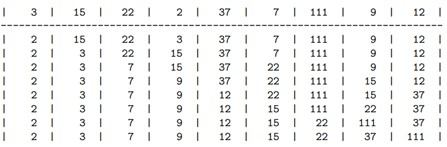
\includegraphics{SelectionSort}
	\break
	
	\textbf{b) Vertausch-Operationen} \hfill \break
	
	Anzahl der in a) geschrieben Zeilen (Achtung minus die erste Zeile)
	
	Anmerkung: Selbstvertauschung tritt auf, wenn das jetzige Element schon an der richtigen Stelle ist.
	\newline
	\newline
	\textbf{c) Vergleichs-Operationen}
	\newline
	\newline
	n: Anzahl der Elemente im Array
	
	\begin{center}
		$Vergleichs \ Operationen = $\Large{$\frac{n(n-1)}{2}$}
	\end{center}
	
	Anmerkung: Egal nach welchem Kriterium sortiert wird, diese Formel gilt immer!
	
	\pagebreak
	
	
	\subsection{Insertion Sort}
	\textbf{a) Sortieren Beispiel}
	
	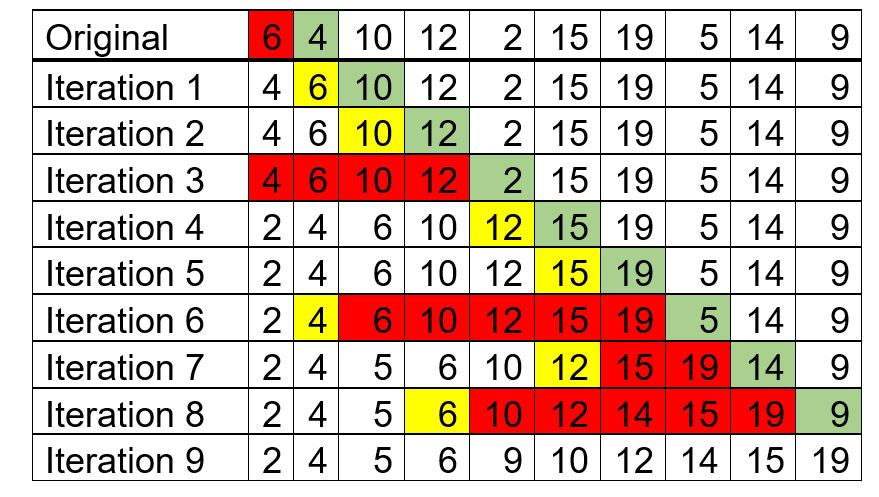
\includegraphics[scale=0.5]{InsertionSort}
	
	\textbf{b) Vertausch-Operationen:} \newline
	1.	Markiere in jeder Zeile die „Vergleichs-Diagonale grün“
	
	2.	Markiere in jeder Zeile rot bis zum Index auf das grün markierte Element
	
	3.	Vertausch-Operationen = Anzahl der roten Elemente\hfill \break
	
	\textbf{c) Vergleichsoperationen:} \newline
	1.	Schritte 1 und 2 von „Vertausch-Operationen“
	
	2.	Markiere, wenn möglich, links ein zusätzliches Kästchen gelb
	
	3.	Vergleichs-Operationen = Anzahl der roten Elemente + Anzahl der gelben Elemente
	
	\newpage
	
	\subsection{Bubble Sort}
	\textbf{a) Sortieren Beispiel}
	\newline\newline
	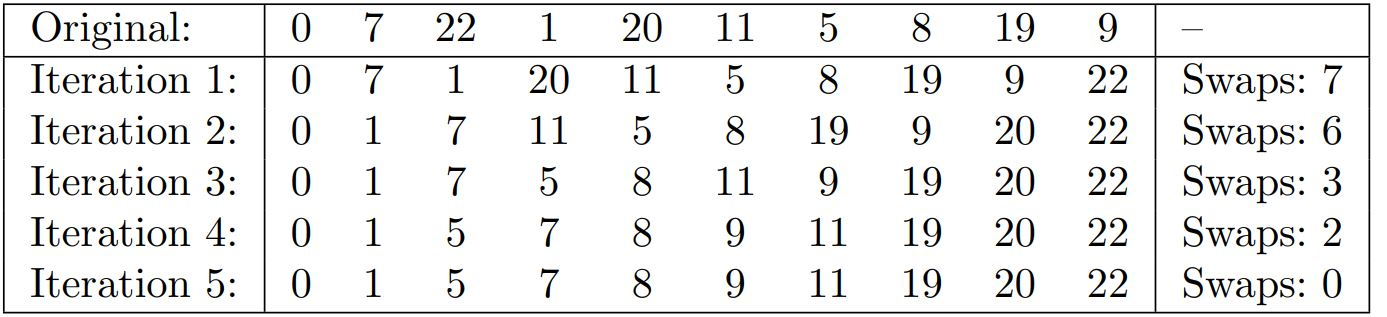
\includegraphics[scale=0.5]{BubbleSort}
	\newline
	
	\textbf{b) Vertausch-Operationen} \newline
	Kein Muster, nur doch durchzählen möglich. \hfill \break
	\newline
	\textbf{c) Vergleichsoperationen}
	

		\begin{center}
		$Vergleichs \ Operationen = selbst geschrieben \ Zeilen * Elemente$
	\end{center}
	
\end{document}
